% debut d'un fichier latex standard
\documentclass[a4paper,12pt,twoside]{article}

% pour l'inclusion de figures en eps,pdf,jpg
\usepackage{graphicx}
\usepackage{subcaption}
\usepackage{wrapfig}
% quelques symboles mathematiques en plus
\usepackage{amsmath}
% le tout en langue francaise
%\usepackage[french]{babel}
% on peut ecrire directement les caracteres avec l'accent
% a utiliser sur Linux/Windows
\usepackage[utf8]{inputenc}
\usepackage[T1]{fontenc}
% a utiliser sur le Mac
%\usepackage[applemac]{inputenc}
% pour l'inclusion de links dans le document
\usepackage[colorlinks,bookmarks=false,linkcolor=blue,urlcolor=blue]{hyperref}
\usepackage{siunitx}
% pour les degrés
\usepackage{textcomp}
\paperheight=297mm
\paperwidth=210mm

\setlength{\textheight}{235mm}
\setlength{\topmargin}{-1.2cm} % pour centrer la page verticalement
%\setlength{\footskip}{5mm}
\setlength{\textwidth}{15cm}
\setlength{\oddsidemargin}{0.56cm}
\setlength{\evensidemargin}{0.56cm}

\pagestyle{plain}

% quelques abreviations utiles
\def \be {\begin{equation}}
\def \ee {\end{equation}}
\def \dd  {{\rm d}}

\newcommand{\mail}[1]{{\href{mailto:#1}{#1}}}
\newcommand{\ftplink}[1]{{\href{ftp://#1}{#1}}}
%
% latex SqueletteRapport.tex      % compile la source LaTeX
% xdvi SqueletteRapport.dvi &     % visualise le resultat
% dvips -t a4 -o SqueletteRapport.ps SqueletteRapport % produit un PostScript
% ps2pdf SqueletteRapport.ps      % convertit en pdf

% pdflatex SqueletteRapport.pdf    % compile et produit un pdf

% ======= Le document commence ici ======

\begin{document}
% Le titre, l'auteur et la date
\title{Heat problem\\{\small Physique Numérique I}\\{\small Rapport 5}}
\date{\today}
\author{Delphine Martres et Damien Korber\\{\small \mail{delphine.martres@epfl.ch} et \mail{damien.korber@epfl.ch}}}

\maketitle
\tableofcontents % Table des matieres


% Quelques options pour les espacements entre lignes, l'identation
% des nouveaux paragraphes, et l'espacement entre paragraphes
\baselineskip=16pt
\parindent=15pt
\parskip=5pt
\newpage


%%%% ON COMMENCE A ECRIRE D'ICI

\section{Introduction}

\begin{wrapfigure}{r}{0.55\textwidth}
 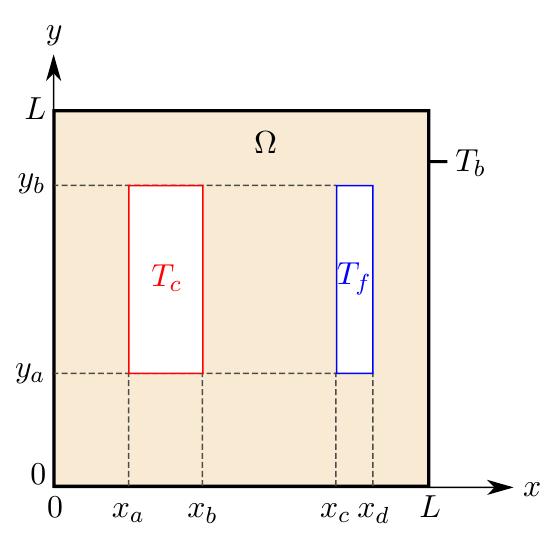
\includegraphics[width=0.45\textwidth]{graphs/schema.png}
 \caption{Geometry of the problem}
 \label{schema}
\end{wrapfigure}


This problem focuses on the propagation of heat in an homogeneous environment.
We consider two rectangular bodies of same height and respective temperatures $T_c = 200$°C and $T_f = -100$°C inside of a square box $\Omega$, of which the outside boundary is at Temperature $T_b = 0$°C. Initially, the temperature of the inside of the box is $T(t=0) = T_b$. The problems satisfies the heat equation \eqref{heateq}:

\begin{equation}
 \frac{\partial T}{\partial t} = D\nabla ^2 T
 \label{heateq}
\end{equation}
with $D=\kappa/(\rho C)=const$, where $\kappa=1.2~\si{\W \per \K \per \m}$ is the thermal conductivity, $\rho=1.2~\si{\kg \per \m^3}$ is the mass density, and $C=10^3~\si{\J \per \kg \per \K}$ is the specific heat capacity.


The geometry of the problem is as represented on Fig.\ref{schema}, where the parameters are: $L=10$ cm, $x_a=2$ cm, $x_b=4$ cm, $x_c=7.5$ cm, $x_d=8.5$ cm, $y_a=3$ cm, and $y_b=8$ cm.

In this report, the evolution of the system with respect to time will be simulated in order to study the heat flux and thermal power of each body.

% TODO : Explication de la dérivation spatiale. (laplacien, ...)

\section{Convergence and stability}

\begin{figure}[h]
  \centering
  \begin{subfigure}[t]{0.45\textwidth}
    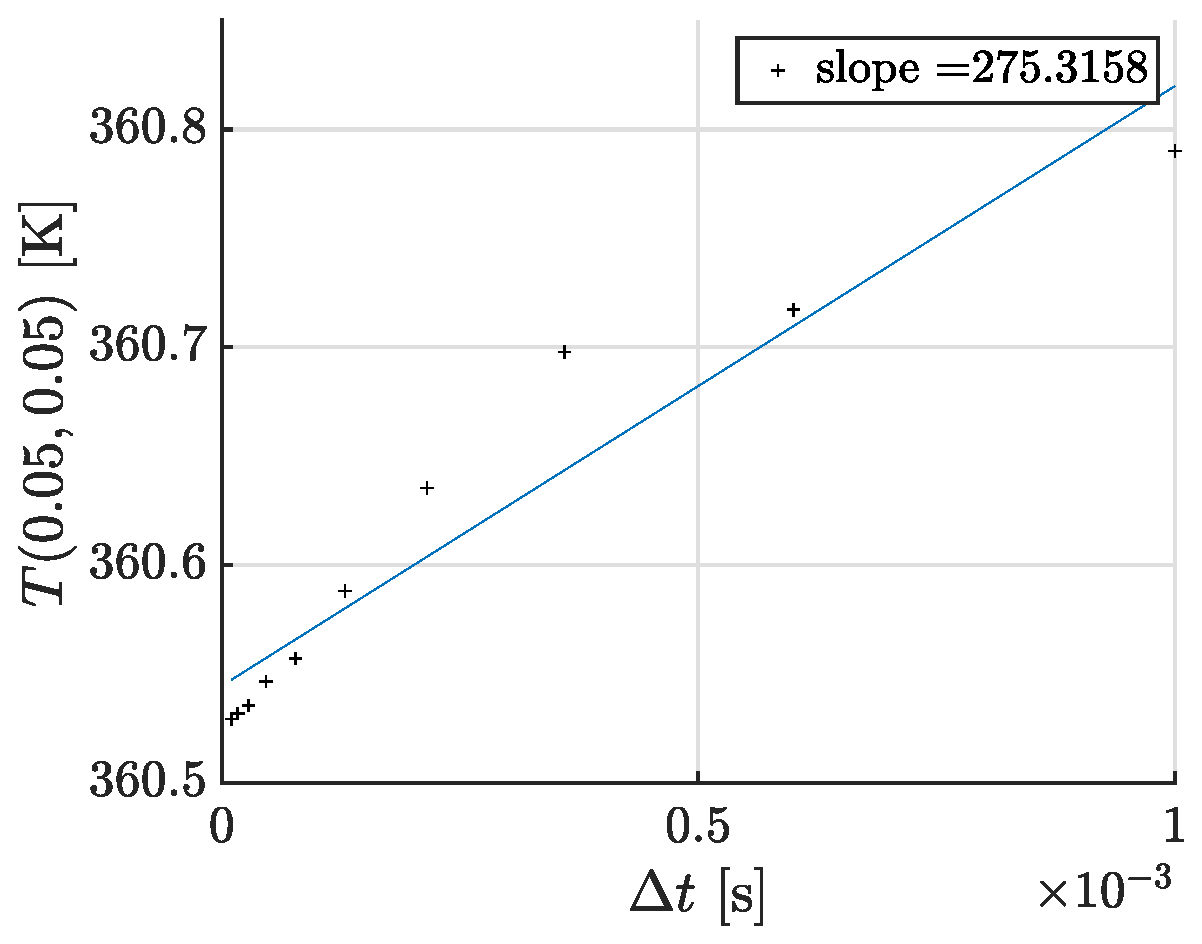
\includegraphics[width=\textwidth]{graphs/b_conv40.eps}

    \caption{Convergence}
    \label{fig:b-conv40}
  \end{subfigure}
  ~
  \begin{subfigure}[t]{0.45\textwidth}
    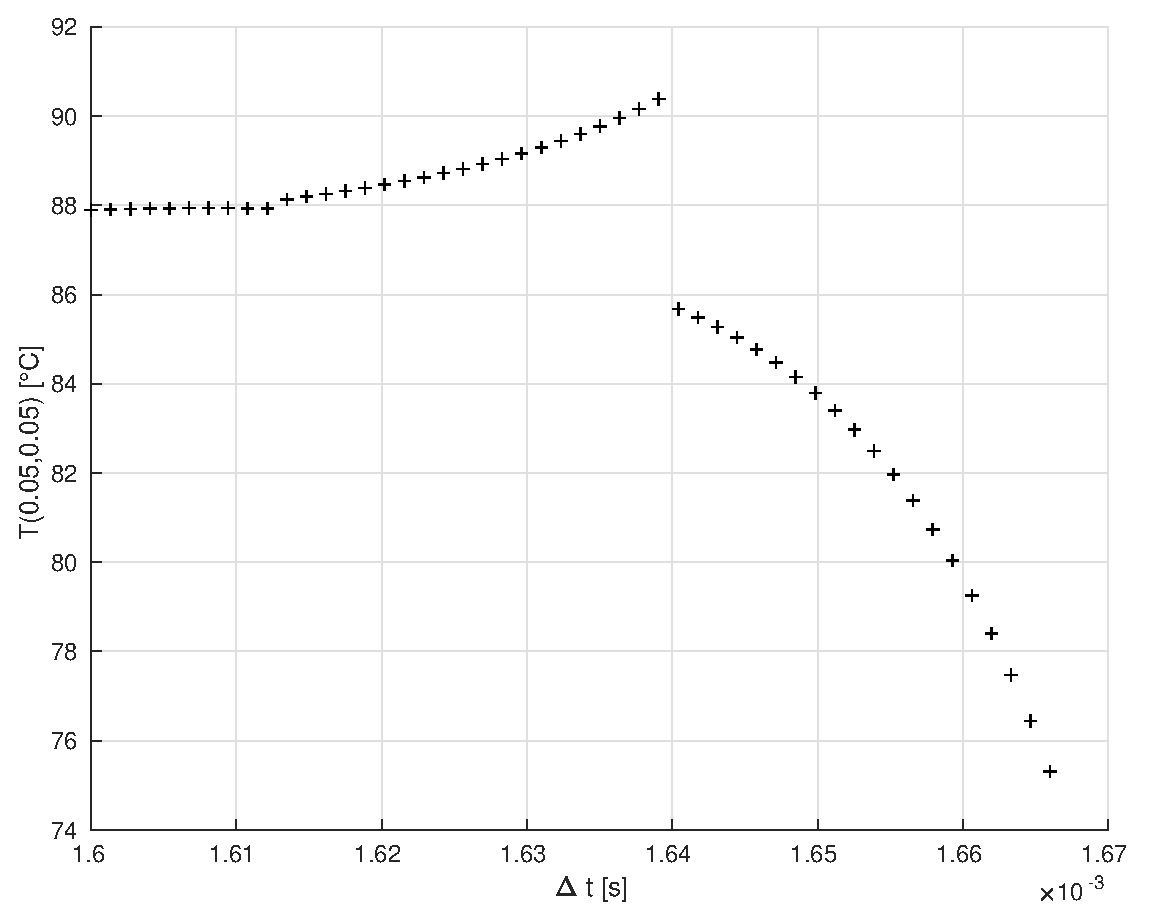
\includegraphics[width=\textwidth]{graphs/b_lim40.eps}
    \caption{Limit of stability}
    \label{fig:b-lim40}
  \end{subfigure}
  \caption{N=40}
  \label{fig:b40}
\end{figure}

\begin{figure}[h]
  \centering
  \begin{subfigure}[t]{0.45\textwidth}
    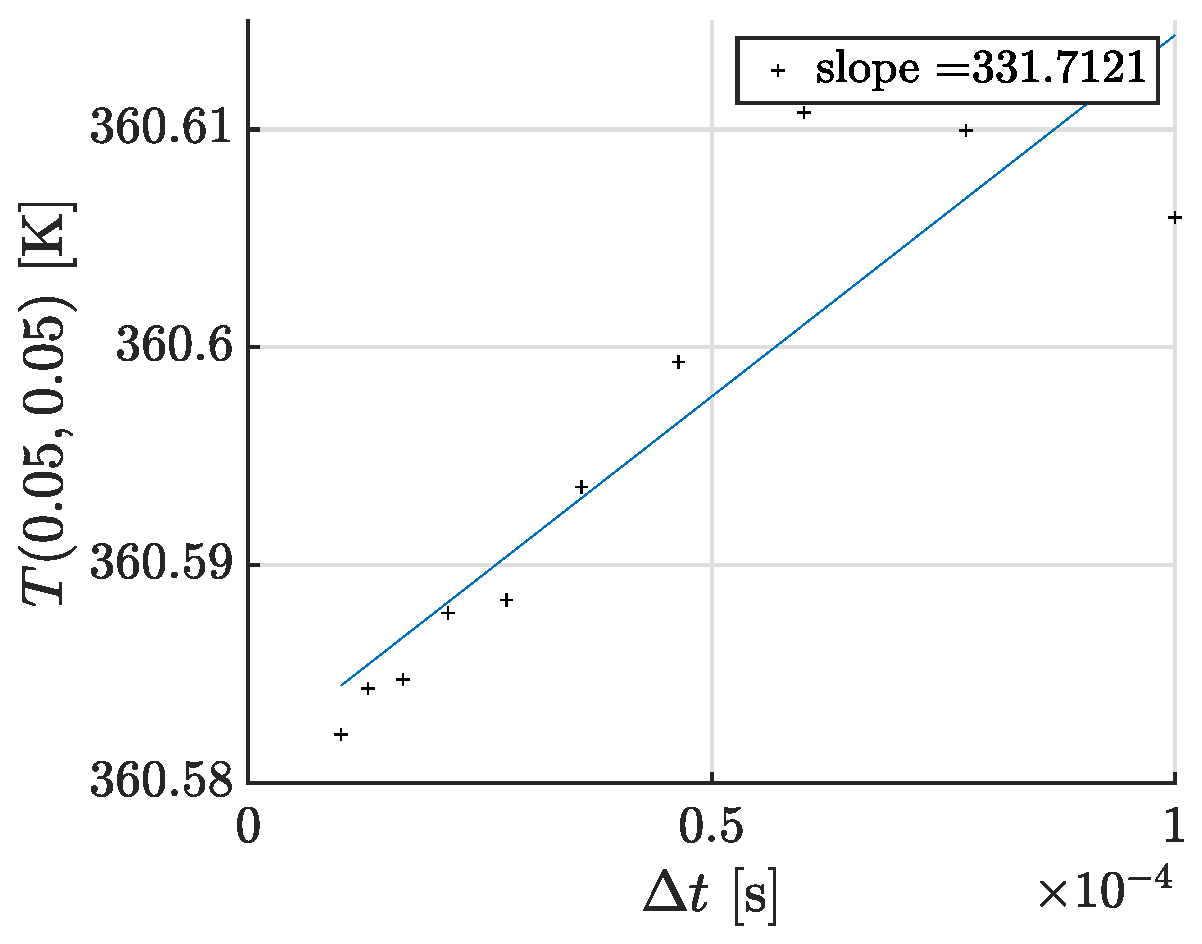
\includegraphics[width=\textwidth]{graphs/b_conv80.eps}

    \caption{Convergence}
    \label{fig:b-conv80}
  \end{subfigure}
  ~
  \begin{subfigure}[t]{0.45\textwidth}
    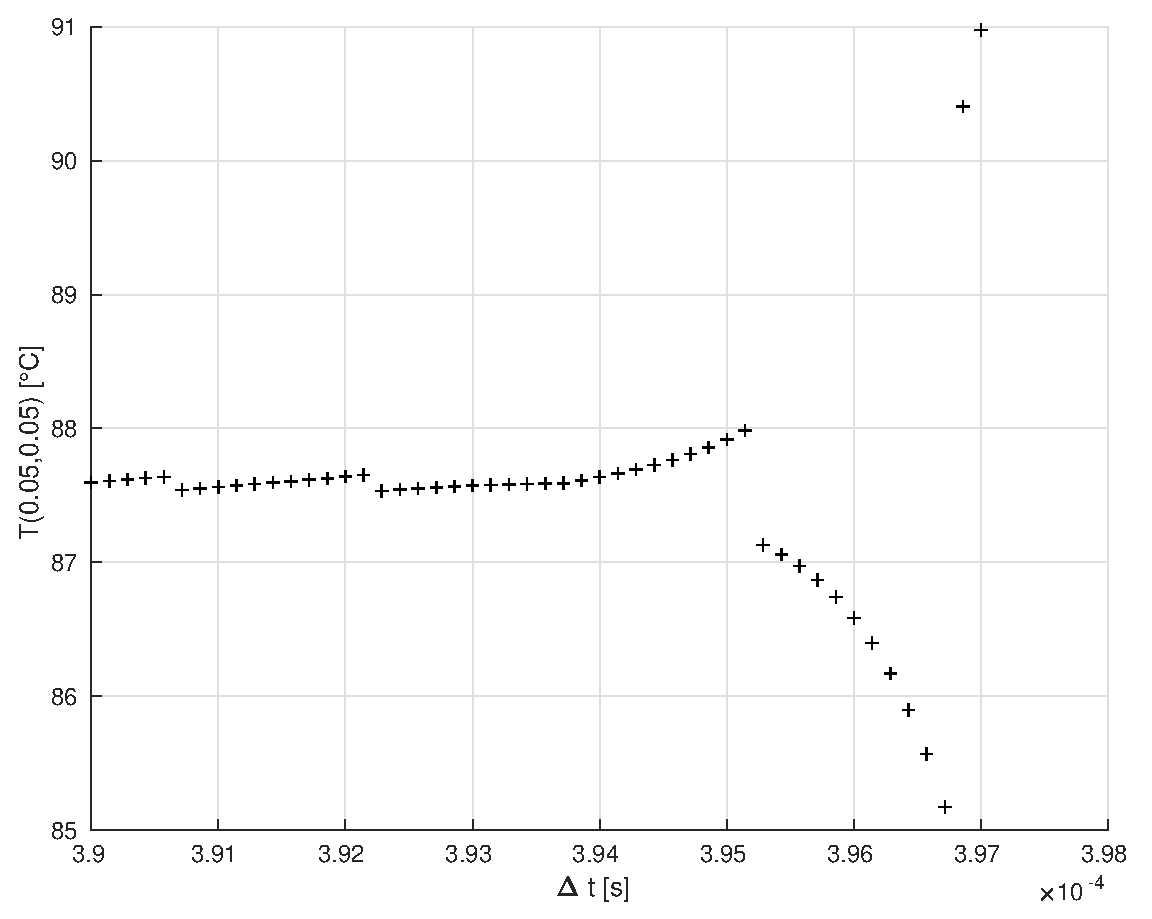
\includegraphics[width=\textwidth]{graphs/b_lim80.eps}
    \caption{Limit of stability}
    \label{fig:b-lim80}
  \end{subfigure}
  \caption{N=40}
  \label{fig:b80}
\end{figure}

\section{Heat flux}
This section focuses on the analysis of the behavious of the heat flux.
The heat flux is obtained with equation \eqref{eq:flux-chaleur}.

\begin{equation}
  \vec{j} = -\kappa\vec{\nabla} T
  \label{eq:flux-chaleur}
\end{equation}

where $\kappa$ is the thermal conductivity.
By using a forward finite difference method, $\vec{j}$ can be numerically computed using equation \eqref{eq:flux-chaleur-numerique}.

\begin{equation}
  \vec{j} = -\frac{\kappa}{h}
  \begin{pmatrix}
    T^k_{i+1,j} - T^k_{i,j} & T^k_{i,j+1} - T^k_{i,j}
  \end{pmatrix}
  \label{eq:flux-chaleur-numerique}
\end{equation}

At $t=\SI{0.1}{\s}$, the flux heat can be seen in two ways, depending on the interest.
On figure \ref{fig:c-temp}, multiple information can be observed.
First, the temperature of the multiple points of the system can be studied using the color gradient.
These colors show the diffusion of heat through the homogeneous environment.
Next, the little arrows show the direction and the intensity of the heat flux.
As it can be observed, the heat flux goes from the hot source to a colder environment.
All of this can be explained by the second law of thermodynamics, which states that in a closed system, entropy never decreases. \cite{wiki:2nd-law}
Thus, the system wants to reach the thermodynamic equilibrum, and heat goes from hot to cold. %TODO : La dernière phrase est pas très belle.

% TODO : Idée - Faire le "spectre" de chaleur sur une bande horizontale.
% The result for the heat flux at $t=\SI{0.1}{\second}$ is given by figures \ref{fig:c-temp} and \ref{fig:c-heat-flux}.

\begin{figure}[h]
  \centering
  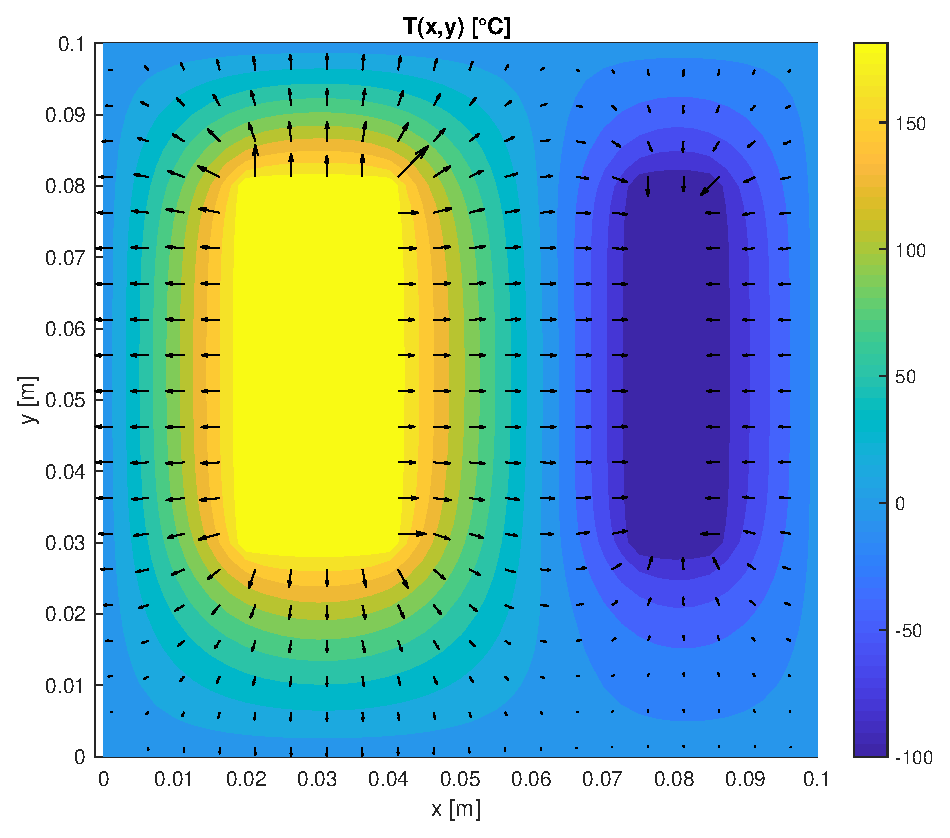
\includegraphics[width=0.6\textwidth]{graphs/c_temp.eps}
  \caption{Graph of temperatures at $t=\SI{0.1}{\s}$, represented by the color gradient, in Kelvin, with the direction and the intensity of the heat flux represented by the arrows.}
  \label{fig:c-temp}
\end{figure}

On figure \ref{fig:c-heat-flux}, the intensity of the heat flux can be observed using the color gradient.
The more yellow it gets, the higher the norm of the heat flux is. %TODO : Phrase pas très belle.
First, the graph shows indirectly the diffusion of heat through the environment.
When the intensity is lower, it either means that the environment is closer to thermodynamic equilibrum or that less heat is flowing. %TODO : Je sais pas si cette phrase a un intérêt, c'est évident.
But the most interesting point on this graph is the corners of the sources, in particular the hot source.
The majority of the environment has a norm for the heat flux around $\SI{10000}{\watt\per\square\meter}$. But on these corners, the norm of the heat flux reaches \SI{25000}{\watt\per\square\meter}.
This behavious does not appear on the border of the heat sources, so it is different from a simple "diffusion".
These are singularities. %TODO : C'est pas un peu fort.
This behavious can be compared to the the \textit{peak effect} \footnote{The name of this effect is directly translated from the french expression: \textit{effet de pointe}. No real translation of this effect in english seems to exist.}, an effect in electrostatics that describes the concentration of charges on the peak of a conductor.
This comparison is not innocent, as there is a mathematical similarity between the electric field and the heat flux.
The electric field $\vec{E}$ is derived from a scalar potential $\phi$, which give equation \eqref{eq:elec-field}.

\begin{equation}
  \vec{E} = \vec{\nabla}\phi
  \label{eq:elec-field}
\end{equation}

Equation \eqref{eq:elec-field} is similar to equation \eqref{eq:flux-chaleur}, as $\vec{j}$ is also derived from a scalar potential ($T$). %TODO : C'est juste de dire que T est un potentiel scalaire ?
Thus, the peaks in intensity on the corners of the sources can be compared to the \textit{peak effect} of electrostatics.

\begin{figure}[h]
  \centering
  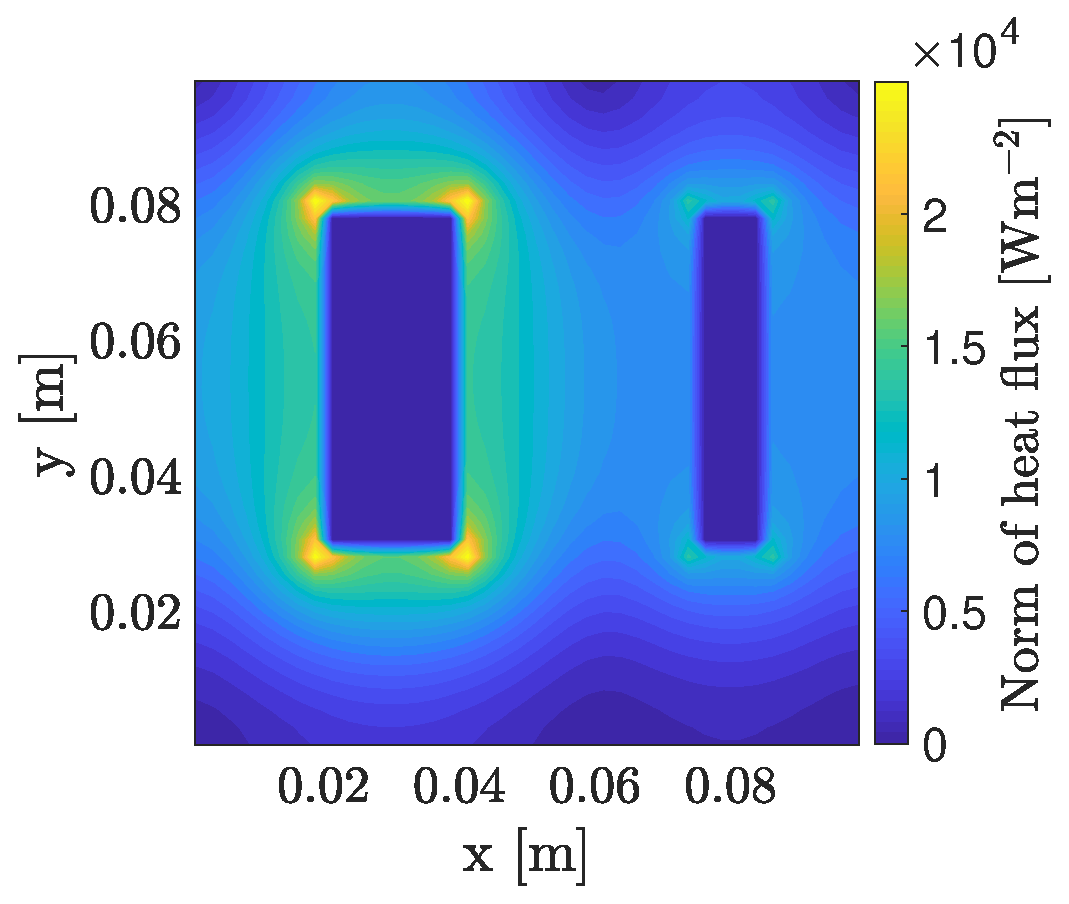
\includegraphics[width=0.6\textwidth]{graphs/c_heat_flux.eps}
  \caption{Intensity of the heat flux represented by the color gradient.}
  \label{fig:c-heat-flux}
\end{figure}
% \begin{figure}[h]
%   \centering
%   \begin{subfigure}[t]{0.45\textwidth}
%     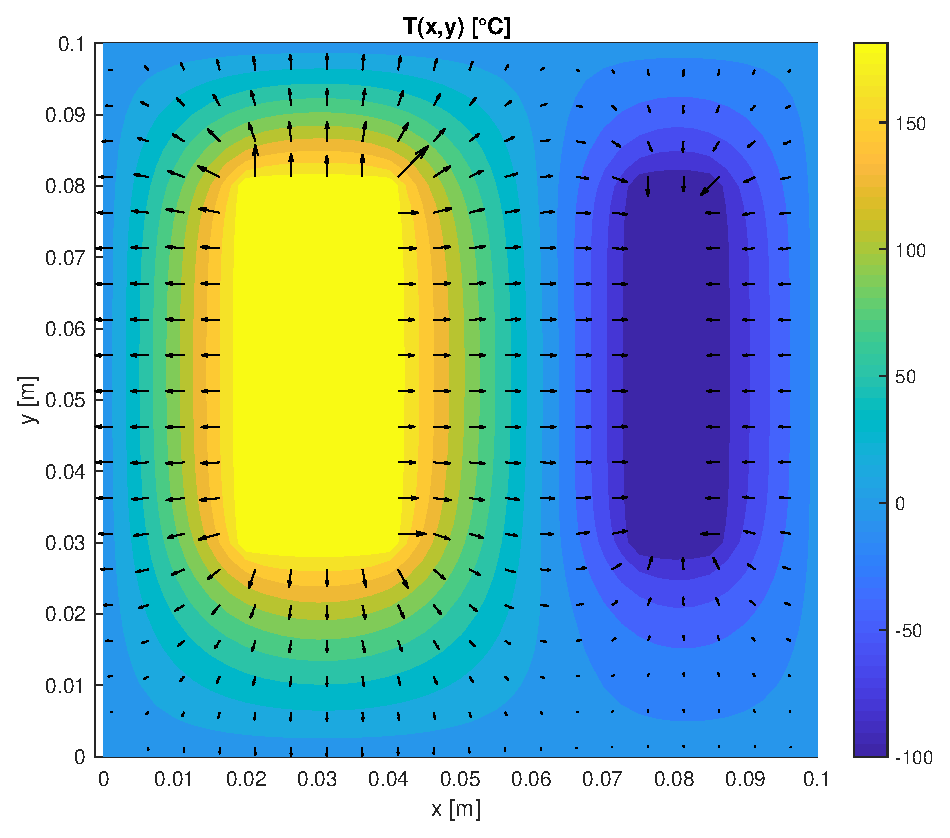
\includegraphics[width=\textwidth]{graphs/c_temp.eps}
%     \caption{Graph of temperatures, represented by the color gradient, in Kelvin, with the direction and the intensity of the heat flux represented by the arrows.}
%     \label{fig:c-temp}
%   \end{subfigure}
%   ~
%   \begin{subfigure}[t]{0.45\textwidth}
%     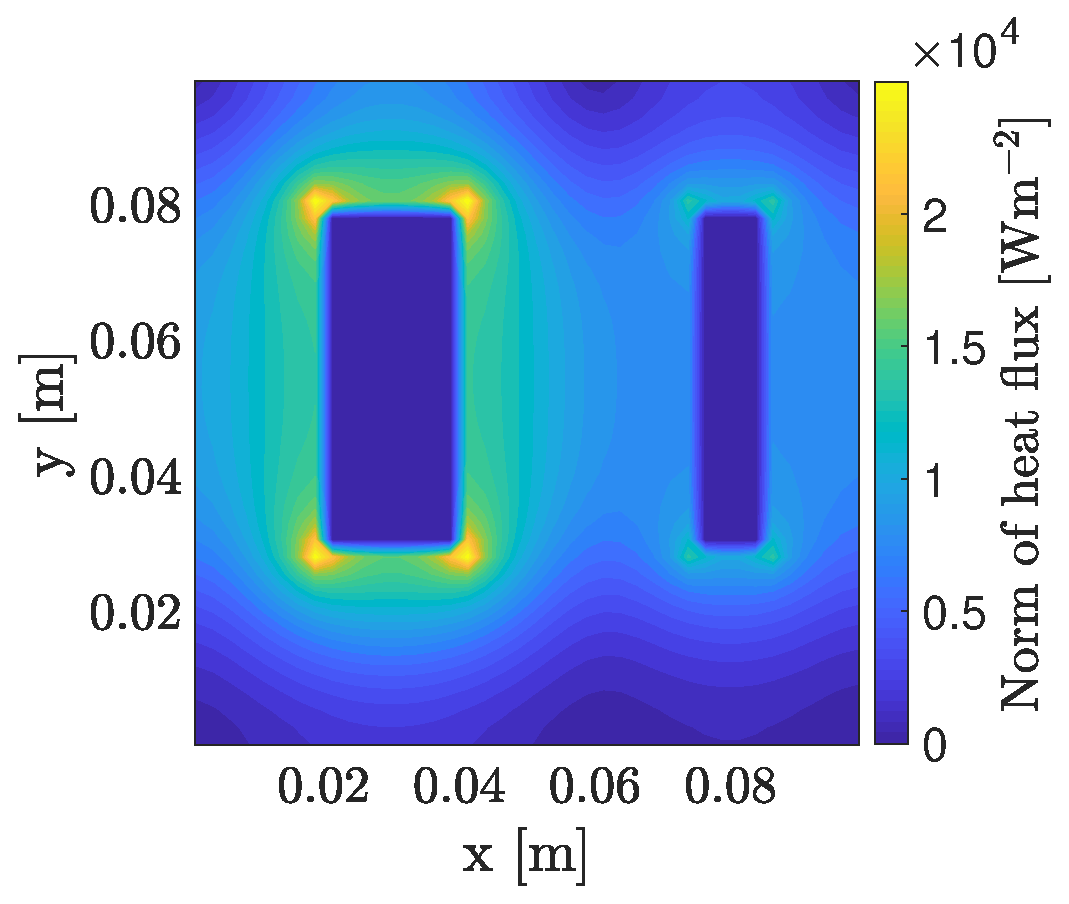
\includegraphics[width=\textwidth]{graphs/c_heat_flux.eps}
%     \caption{Intensity of the heat flux represented by the color gradient.}
%     \label{fig:c-heat-flux}
%   \end{subfigure}
%   \caption{Study of the heat flux at $t=\SI{0.1}{\second}$.}
%   \label{fig:c}
% \end{figure}

\section{Power}

\section{Heat flux with respect to the distance between the bodies}

\begin{figure}[h]
  \centering
  \begin{subfigure}[t]{0.45\textwidth}
    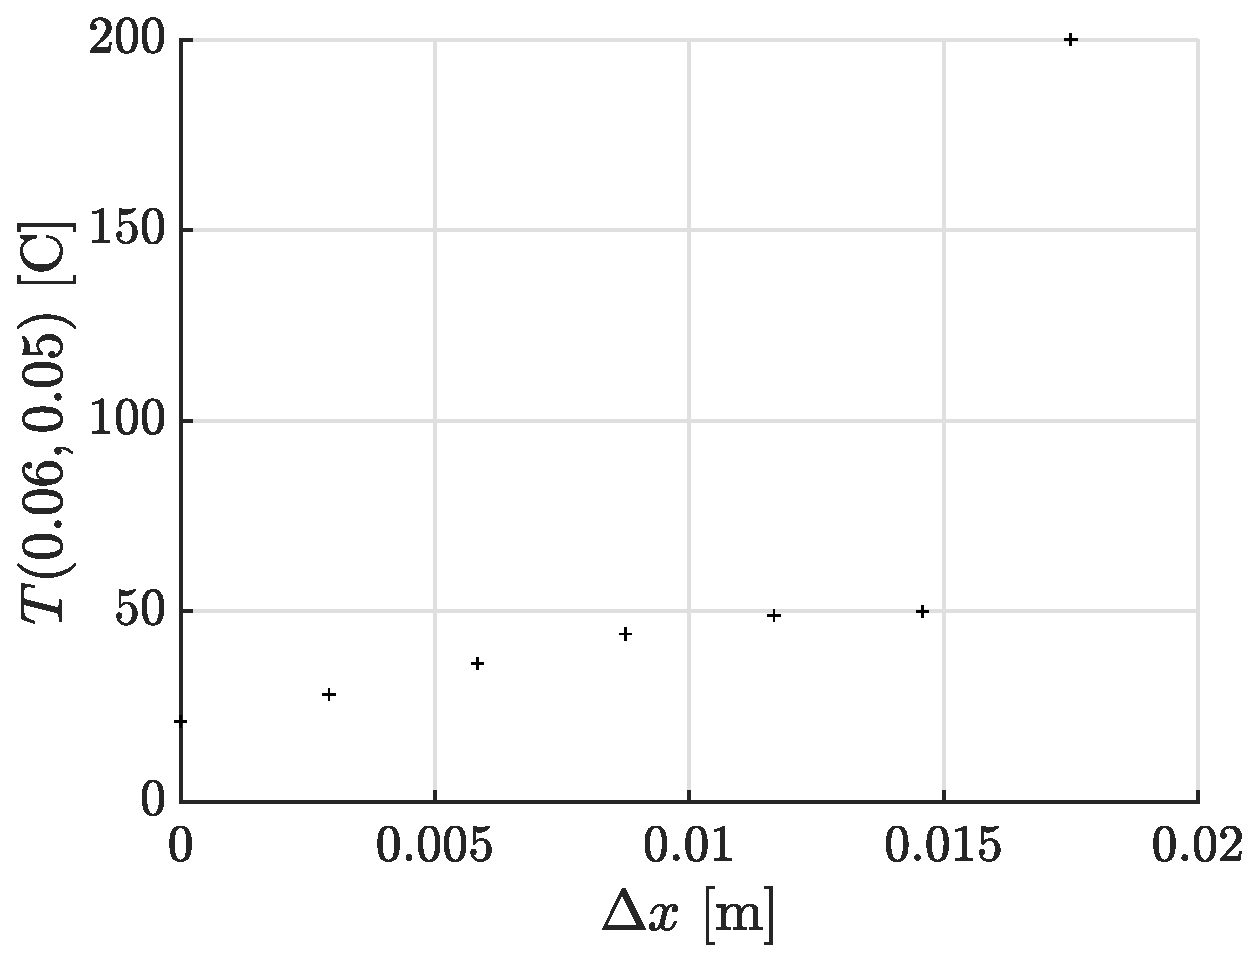
\includegraphics[width=\textwidth]{graphs/e_distT.eps}
    \caption{Temperature}
    \label{fig:e-T}
  \end{subfigure}
  ~
  \begin{subfigure}[t]{0.45\textwidth}
    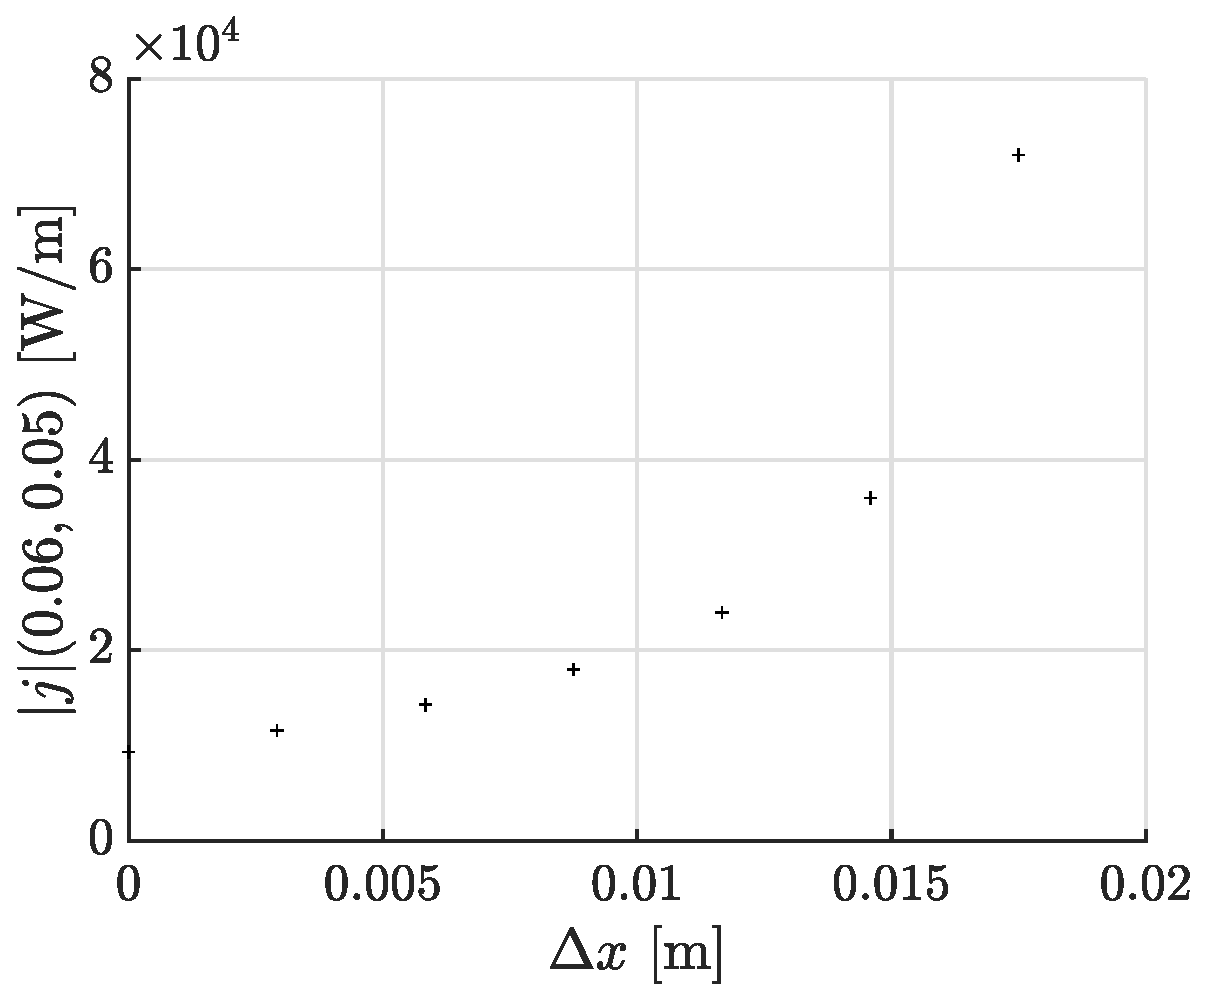
\includegraphics[width=\textwidth]{graphs/e_distF.eps}
    \caption{Heat flux}
    \label{fig:e-T}
  \end{subfigure}
  \caption{Temperature and heat flux in function of displacement}
  \label{fig:e}
\end{figure}

\section{Conclusion}

\begin{thebibliography}{99}
  \bibitem{wiki:2nd-law} Wikipedia contributors, "Second law of thermodynamics," Wikipedia, The Free Encyclopedia, \url{https://en.wikipedia.org/w/index.php?title=Second_law_of_thermodynamics&oldid=884867223} (accessed March 2, 2019).


\end{thebibliography}

\end{document}
